%%
%% Author: ncw135
%% 13/05/2019
%%

% Preamble
\documentclass[11pt]{article}

% Packages
\usepackage{amsmath}
\usepackage{graphicx}
\usepackage[a4paper]{geometry}
\usepackage{cleveref}
\usepackage{subcaption}
% Document

\title{Task2: Parameter estimation}
\begin{document}
\maketitle
    In task1 you built a model from a full description of the topology, initial conditions and parameters. This
    time you are given the topology and some experimental data, but you will have to find the parameters yourself. Its
    a good idea, when you get time, to read some literature on parameter estimation of ODE models. Its not essential,
    since mostly Copasi takes care of the details, but it is helpful to have at least a rudimentary understanding of
    what is going on...

    In model 2, A is activated by the presence of S with Hill kinetics. Hill kinetics are a common way of modelling
    receptor activation. Then we have a small phosphorylation cascade starting at Ap which activates B which in turn
    activates C. Both forwards and backwards reactions in this chain of phosphorylations follow michaelis-menten
    kinetics, except for the activation of B which is instead competitively inhibited by I. Note that the competitive
    inhibition rate law converges to the michaelis menten when the inhibitor is not present. Furthermore,
    phosphorylated C enhances the dephosphorylation of A, thereby completing a negative feedback loop.

    \begin{figure}[h]
        \centering
        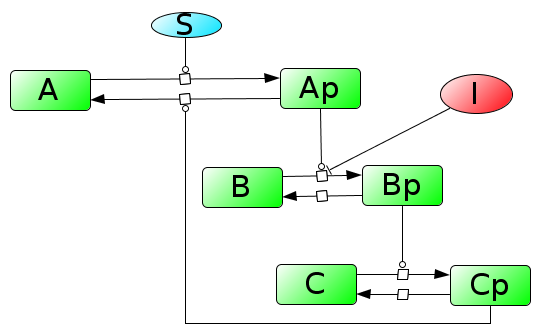
\includegraphics[width=0.9\textwidth]{figures/Model2.png}
        \caption{Network topology for model 2. }
    \end{figure}


    \begin{enumerate}
        \item You have a file containing experimental data that will fit this model. Use matplotlib and seaborn PythonForScience packages to visualise these data
        \item Build the model topology using antimony
        \item Use Copasi to setup a parameter estimation that estimates all of the parameters of this model
        \begin{itemize}
            \item Use what you know about the model from the experimental conditions
            \item Consider which algorithm to use, as well as the hyperparameters
            \item Consider how to weight the objective function.
        \end{itemize}
        \item Use PyCoTools to configure and run the same parameter estimation
        \item Use PyCoTools to run several parameter estimations simultaneously
        \item Use PyCoTools to run many parameter estimations on the cluster
        \item Use PyCoTools to configure and run an identifiability analysis (profile likelihoods) on the cluster
    \end{enumerate}

    Do a small bit of background reading version control and git/github. There's no need to go mad
    as Git is one of those things that you learn little by little, as and when new functions are needed -- most notably
    when you accidentally destroy your program and want to revert to a previous state. Then:

    \begin{enumerate}
        \item Create a new git repository for the code you have generated so ofar
        \item Add your files to the repository and commit your progress
        \item Push your repository to the Git servers
        \item Change something in your project (literally anything)
        \item Use `git status` in the terminal to see that git has tracked your changes
        \item Use the git add, git commit and git push commands to make your changes permanent.
    \end{enumerate}




\end{document}